% Project 2 - EECS 499
% Author: Shaun Howard (smh150@case.edu)
\documentclass[conference]{IEEEtran} \usepackage[T1]{fontenc} \usepackage[backend=biber, style=ieee]{biblatex}
\addbibresource{report.bib} \usepackage[final]{microtype}

% graphics
\ifCLASSINFOpdf \usepackage[pdftex]{graphicx} % declare the path(s) where your graphic files are
  \graphicspath{{images/}} % and their extensions so you won't have to specify these with
  % every instance of \includegraphics
  \DeclareGraphicsExtensions{.jpeg,.png} \else
\fi


\begin{document}

\title{Randomized Potential Field Motion Planning for Baxter Dual Arm Manipulator}

\author{
 \IEEEauthorblockN{Shaun Howard}
 \IEEEauthorblockA{Electrical Engineering and Computer Science Department\\
                   Case Western Reserve University\\ 
                   Cleveland, Ohio 44106\\
                   Email: smh150@case.edu}

% make the title area
\maketitle

% As a general rule, do not put math, special symbols or citations
% in the abstract
\begin{abstract}

\end{abstract}

\section{Introduction} \label{Introduction}

\begin{figure}
\label{pic1} 
\centering 
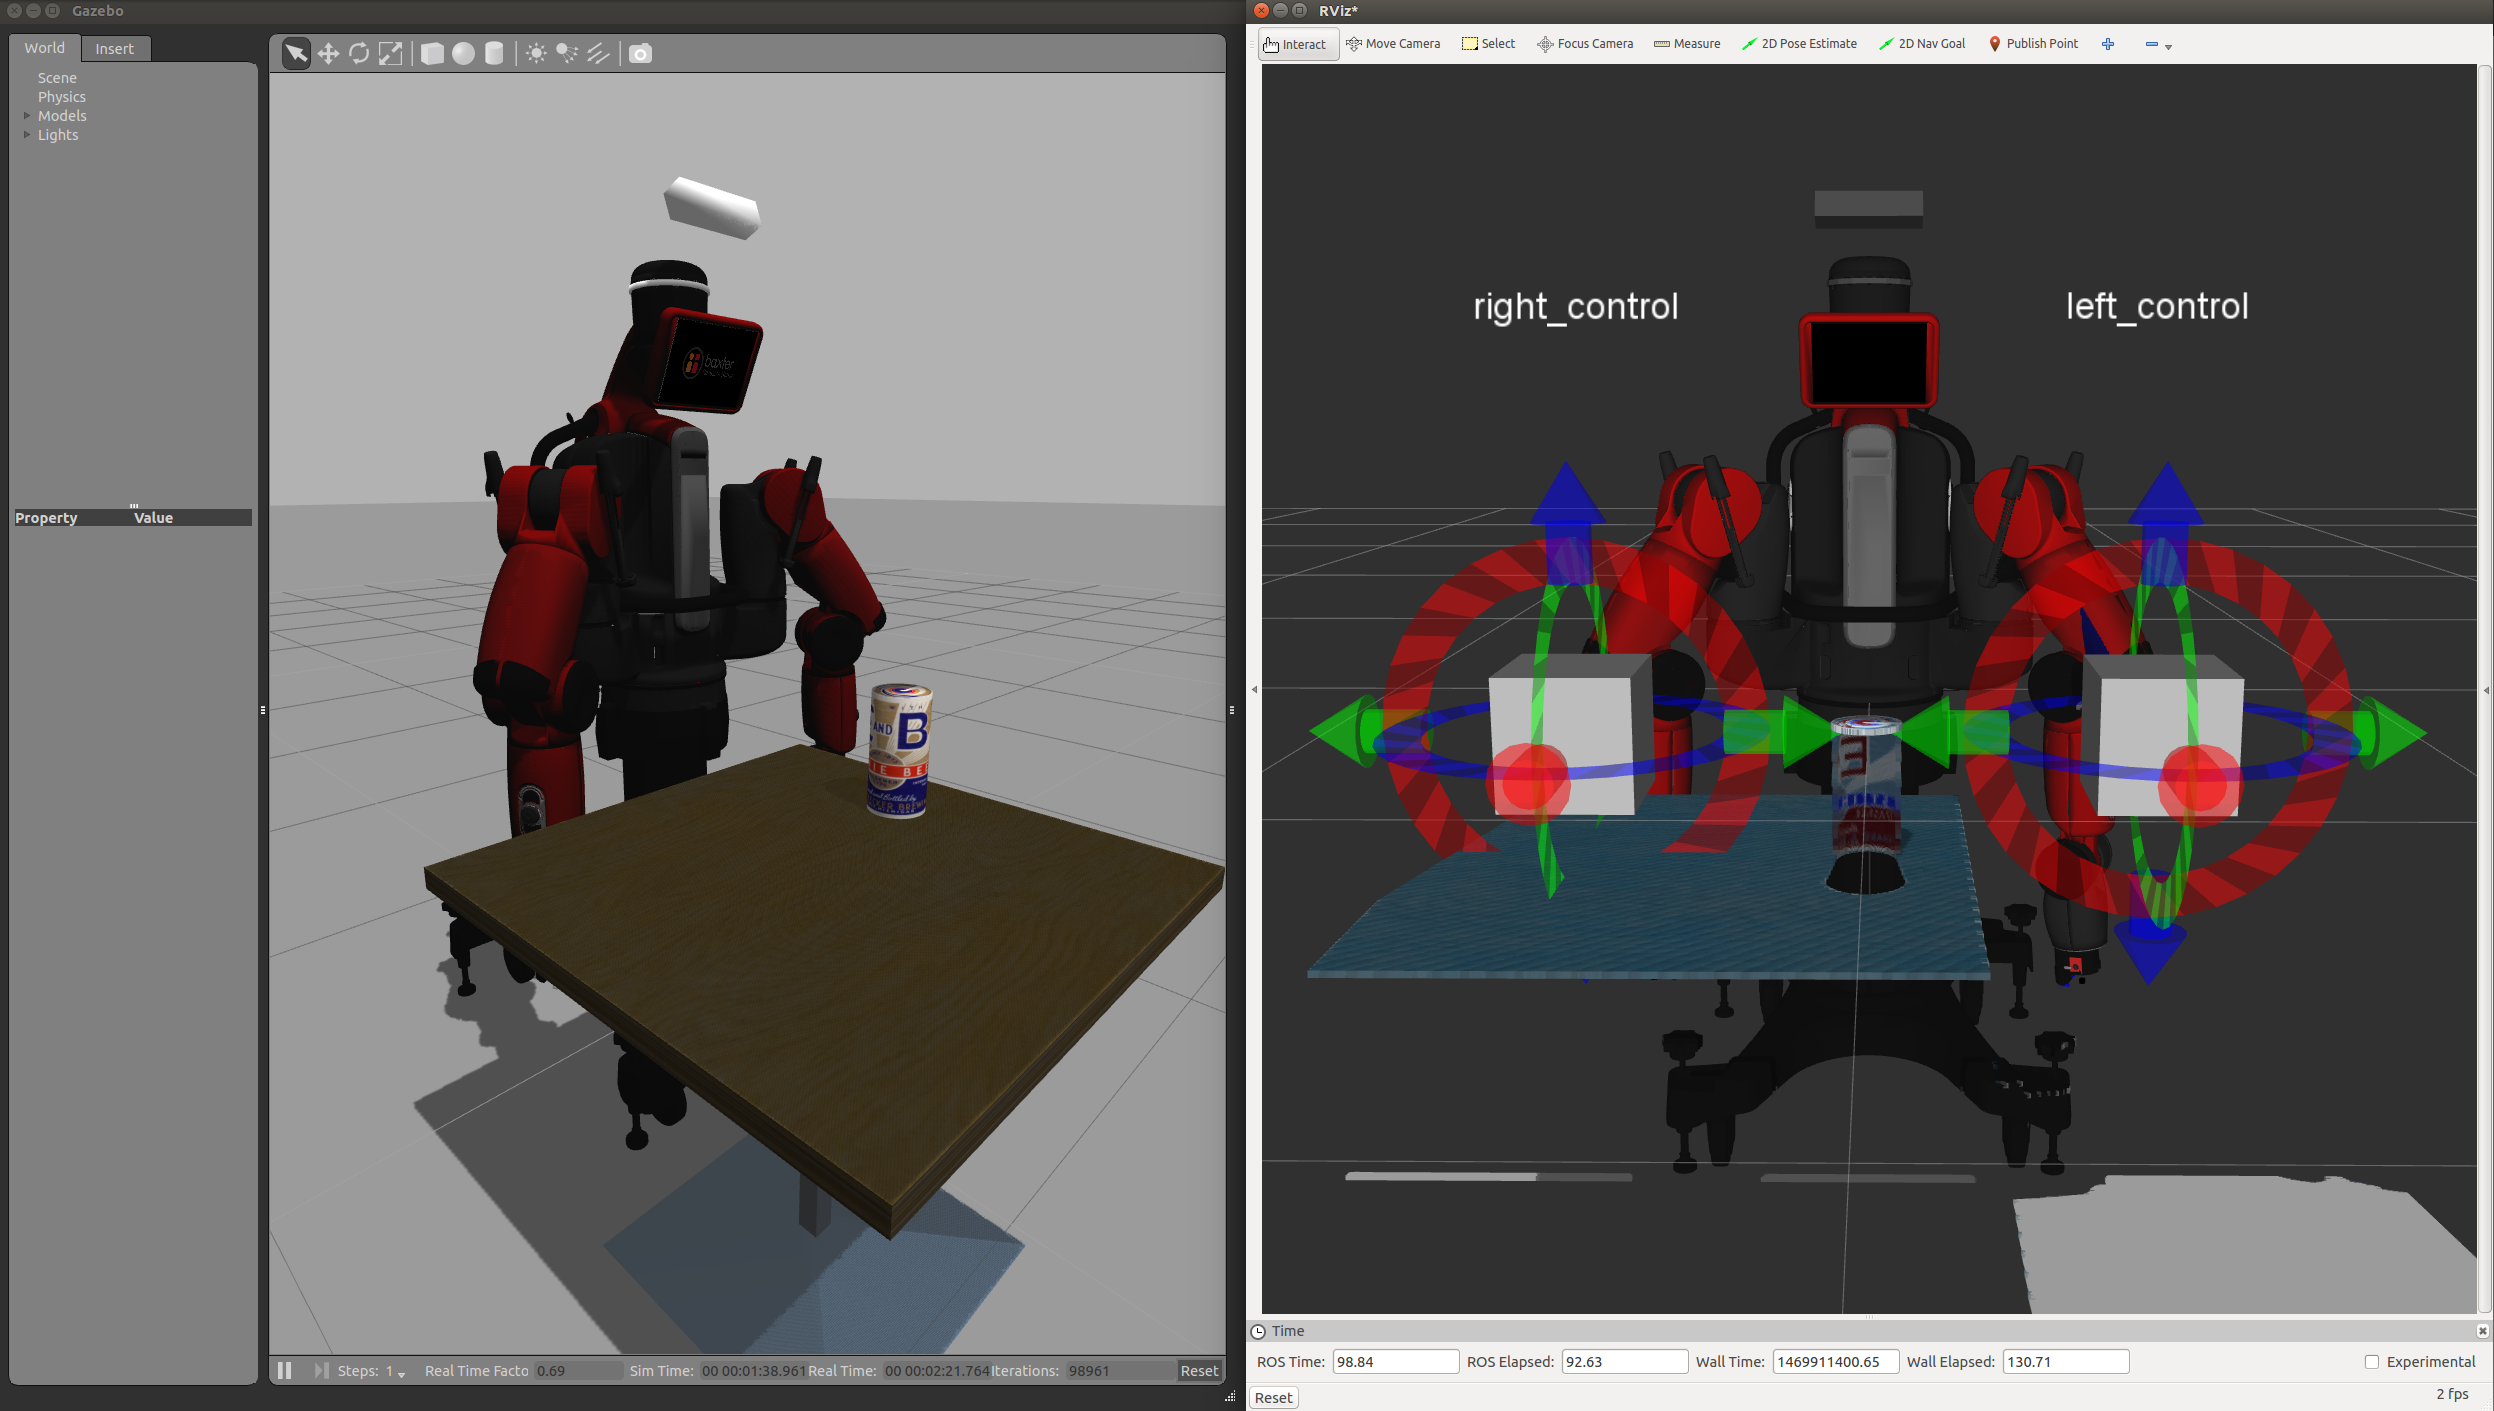
\includegraphics[width=0.49\textwidth]{sim1}
\caption{A squadron S of three TurtleBot 2's on a grid-based world attempt to estimate the position of R, the middle moving TurtleBot 2.}
\end{figure}

\section{Related Work} \label{Related Work}

\section{Problem Formulation} \label{Problem Formulation}

\section{Methodology} \label{Methodology}

\subsection{Sensor Measurements} \label{Sensor Measurements}

\subsection{Planner Implementation} \label{Planner Implementation}

\subsection{Gazebo Simulation} \label{Gazebo Simulation}

\section{Conclusion} \label{Conclusion} 

\subsection{Future Work}

\printbibliography
\end{document}